\documentclass{article}

\usepackage{microtype}
\usepackage{graphicx}
\usepackage{booktabs}
\usepackage{amsmath}
\usepackage{amssymb}
\usepackage{hyperref}
\usepackage{enumitem}
\usepackage{xcolor}
\usepackage{tikz}
\usepackage{pgfplots}
\usepackage{placeins}
\usepackage{algorithm}
\usepackage{algorithmic}

\usetikzlibrary{arrows.meta,positioning}
\pgfplotsset{compat=1.18}
\makeatletter
\setlength{\@fptop}{0pt}
\setlength{\@dblfptop}{0pt}
\setlength{\@fpsep}{8pt plus 1pt}
\setlength{\@dblfpsep}{8pt plus 1pt}
\makeatother
\newcommand{\repairkv}{\textsc{RepairKV}}
\newcommand{\bbase}{\ensuremath{B_{\mathrm{base}}}}
\newcommand{\bmatch}{\ensuremath{B_{\mathrm{match}}}}
\newcommand{\spanref}{\ensuremath{\mathrm{SpanRef}\mbox{-}K}}

\usepackage{icml2026}

\icmltitlerunning{Cache Me if You Can: Repairing the KV State after Compression}

\begin{document}

\twocolumn[
  \icmltitle{Cache Me if You Can: Repairing the KV State after Compression}

  \begin{icmlauthorlist}
    \icmlauthor{Andrew Rusli}{equal,harvard}
    \icmlauthor{Shreyan Paliwal}{equal,harvard,opt32}
  \end{icmlauthorlist}
  \icmlaffiliation{equal}{Equal contribution}
  \icmlaffiliation{harvard}{Harvard College, Cambridge, MA, USA}
  \icmlaffiliation{opt32}{Opt32}
  \icmlcorrespondingauthor{Shreyan Paliwal}{shreyanpaliwal@college.harvard.edu}
  \icmlkeywords{resource-adaptive inference, dynamic KV cache compression,
    KV cache repair, cross-turn relevance shift, quality-resource tradeoffs}
  \vskip 0.3in
]

\printAffiliationsAndNotice{\icmlEqualContribution}

\begin{abstract}
  As large language models (LLMs) support longer contexts and more capable agentic sessions, what matters in the accumulated context can change with each new query, tool output, test result, or browser observation.
  At the same time, inference still depends on a limited active key-value (KV) cache, and many existing KV-cache compression methods decide which past tokens stay active from the current prefix.
  As a result, tokens that matter in later turns may already have been evicted or compressed away in earlier compression decisions. 
  We study post-compression KV cache repair, a runtime mechanism that restores previously evicted tokens to the active cache.
  \repairkv{} uses the interval between turns to reevaluate which tokens are important from evicted KV rows stored in a slower memory tier, then promotes a small subset before decoding resumes.
  Controlled experiments show that this recovery persists when relevance changes and across different initial eviction policies (compression styles), and a preliminary diagnostic on open-source repositories shows the same pattern; on Qwen2.5-7B-Instruct at 32K context, \repairkv{} achieves 91.0\% retrieval on a four-query needle-in-a-haystack task versus 24.5\% for the matched no-repair baseline at the same active-cache budget, with only 96 promoted tokens. 
\end{abstract}
 
% -----------------------------------------------------------------------
\section{Introduction}
% -----------------------------------------------------------------------

\paragraph{Motivation.}
Long-context inference increasingly depends on KV-cache compression and
offload.
During decoding, a transformer stores key-value (KV) activations for prior
tokens so later tokens can attend to them.
The model weights are fixed once loaded, but the KV cache grows with the
number of tokens kept for each live sequence; at long context lengths, this
sequence-dependent state can dominate available GPU memory and increase
inference-time attention and cache-management costs.
KV-cache compression and offload reduce this pressure by deciding which
historical state remains active on GPU and which state is evicted or moved
to a slower tier.
That decision is usually made with information available at the current
turn, so it is often treated as a one-way operation: evict now, decode
later from the retained active set.

\begin{figure}[t]
\centering
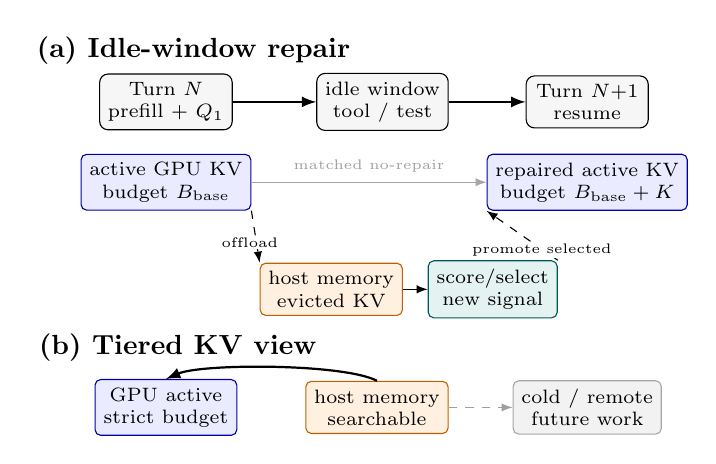
\begin{tikzpicture}[font=\scriptsize, >=latex,
  stage/.style={draw, rounded corners=3pt, align=center, inner sep=3pt,
                minimum width=1.55cm, minimum height=0.5cm, fill=gray!7},
  gpu/.style={draw=blue!65!black, fill=blue!8, rounded corners=2pt,
              align=center, inner sep=3pt, minimum width=1.7cm},
  host/.style={draw=orange!75!black, fill=orange!12, rounded corners=2pt,
               align=center, inner sep=3pt, minimum width=1.7cm},
  signal/.style={draw=teal!70!black, fill=teal!10, rounded corners=2pt,
                 align=center, inner sep=3pt, minimum width=1.55cm},
  cold/.style={draw=gray!70, fill=gray!10, rounded corners=2pt,
               align=center, inner sep=3pt}]
  \node[font=\bfseries] at (1.35,4.45) {(a) Idle-window repair};
  \node[stage] (t0) at (1.0,3.8) {Turn $N$\\prefill + $Q_1$};
  \node[stage] (idle) at (3.75,3.8) {idle window\\tool / test};
  \node[stage] (t1) at (6.35,3.8) {Turn $N{+}1$\\resume};
  \draw[->, thick] (t0) -- (idle);
  \draw[->, thick] (idle) -- (t1);

  \node[gpu] (base) at (1.0,2.78) {active GPU KV\\budget $\bbase$};
  \node[host] (warm) at (3.1,1.42) {host memory\\evicted KV};
  \node[signal] (sig) at (5.15,1.42) {score/select\\new signal};
  \node[gpu] (repair) at (6.35,2.78) {repaired active KV\\budget $\bbase+K$};
  \draw[->, dashed] (base.south east) -- (warm.north west)
    node[pos=0.48, below, xshift=-2pt, font=\tiny, fill=white, inner sep=0.6pt]{offload};
  \draw[->] (warm) -- (sig);
  \draw[->, dashed] (sig.north east) -- (repair.south west)
    node[pos=0.38, below, xshift=4pt, font=\tiny, fill=white, inner sep=0.6pt]{promote selected};
  \draw[->, gray!70] (base.east) -- (repair.west)
    node[midway, above, font=\tiny, text=gray!75]{matched no-repair};

  \node[font=\bfseries] at (1.15,0.68) {(b) Tiered KV view};
  \node[gpu, minimum width=1.8cm] (gpurow) at (1.0,-0.08) {GPU active\\strict budget};
  \node[host, minimum width=1.8cm] (hostrow) at (3.68,-0.08) {host memory\\searchable};
  \node[cold, minimum width=1.8cm] (coldrow) at (6.35,-0.08) {cold / remote\\future work};
  \draw[->, thick] (hostrow.north) .. controls (3.25,0.48) and (1.45,0.48) .. (gpurow.north);
  \draw[->, dashed, gray!75] (hostrow) -- (coldrow);
\end{tikzpicture}
\caption{\repairkv{} System Overview: paused-request KV state repair.
A paused request offloads evicted KV to host memory, scores and promotes a budgeted subset conditioned on the chosen signal $s$, and exposes a conceptual tiered-memory interface that production
engines would materialize through page or block allocators.}
\label{fig:pipeline}
\end{figure}

This static view misses two facts about multi-turn inference.
First, attention relevance is query- and context-dependent: later turns,
retrieved documents, tool outputs, test failures, or file changes can make
previously low-priority context newly important.
Query-aware and fine-grained KV retrieval systems show that both token
criticality and attention-distribution patterns can change with the active
query~\citep{quest,fier}.
Second, agentic workflows often contain non-decoding intervals while the
model waits for external results.
Recent systems make this operationally visible: Continuum schedules
multi-turn agent requests around tool-call gaps and KV-cache lifetimes,
while AgentServe targets local agent serving under tight GPU memory
budgets~\citep{continuum,agentserve}.
These systems show that turn boundaries, cache lifetime, and tool-call waits
are now explicit systems objects, but they preserve or schedule cached state
rather than repairing an already-compressed active cache using the next-turn
signal.

Coding-agent measurements reinforce why this interval is worth studying:
OS-level execution, including tool calls and setup, can account for
56--74\% of task latency~\citep{agentcgroup}.
Furthermore, modern production serving stacks such as
vLLM~\citep{vllm} now deploy prefix caching by default, but re-deriving
evicted KV through a fresh prefill pass remains the fallback on cache
miss, eviction, or paused-request discard.
The cost is severe: prior work reports recompute consuming as much as
99\% of multi-turn prefill time when historical KV is repeatedly
recomputed~\citep{cachedattention}, and 37\% of end-to-end execution
time when paused-request KV is discarded in agentic
workloads~\citep{infercept}, which motivates tiered KV systems that trade
recompute for offloaded reuse~\citep{lmcache,ttkv}.
Together, these factors motivate repairing the active KV state before the next decode.

This paper asks whether a runtime can improve the cache state seen by the
next decode after compression has already run.
Compression is not only a storage-saving step: it decides which past tokens
remain immediately available.
At a pause boundary, the runtime may hold a compressed active cache plus
a host-memory (CPU DRAM) tier of evicted KV rows,
along with a newly available signal $s$.
In shared serving this interval is a scheduler tradeoff; in the
single-session or dedicated setting we target, it is often an idle window for
the paused request.
The central question is whether, given a budget $K$ and any available signal
$s$, the runtime can promote evicted KV rows to improve next-decode quality
under the same resumed active-cache budget.

\paragraph{Setting.}
Recent analysis shows that KV compression can sharply degrade
instructions and facts that later become important~\citep{pitfalls}.
The missing evaluation question is not simply whether compression loses
information, or whether a serving system can preserve state across a pause.
It is whether future-turn information can improve an already-compressed
cache under the same resumed active-cache budget.
A useful benchmark for this question needs explicit turn boundaries, a
hidden future query, shared pre-turn history, and no-repair controls matched
on resumed-cache budget $\bbase+K$.
In our experiments, the future relevance signal is an explicit second-turn
($Q_2$) retrieval query so that the repair effect is measurable, while the
intended workflow claim is broader than query answering.

\paragraph{Contributions.}
\repairkv{} is an inference-time adaptation operator for tiered KV state,
conditioned on the newly available next-turn signal.
The adaptation is non-parametric: model weights, prompts, and decoding
settings are fixed, while the active cache state is revised under a
resource budget.
After turn $N$, the runtime compresses the evictable context portion to
an active set $C_{\mathrm{base}}$ with $|C_{\mathrm{base}}|=\bbase$ and
retains evicted KV in host memory as $W_N$.
When the turn-$(N{+}1)$ signal arrives, \repairkv{} scores that store and
promotes a subset $S_K(Q_2)\subseteq W_N$, $|S_K|\le K$, back into the
active GPU cache before decoding resumes.
Unlike pause/resume serving or within-turn query-aware compression, \repairkv{}
changes a paused, already-compressed cache without rerunning full-prefix
selection.
We contribute:
\begin{itemize}[leftmargin=1.4em,noitemsep,topsep=2pt]
  \item a matched resumed active-cache-budget protocol for the
  post-compression, pre-resume lifecycle stage, isolating cache repair
  from simply keeping more active tokens.
  \item calibrated evidence on pooled split-query multi-query
  needle-in-a-haystack (MQ-NIAH) 4Q/6Q/8Q evaluations, a five-turn
  revisit diagnostic, three first-stage eviction policies, a
  Scissorhands-style persistence stress test, and preliminary
  real-repository diagnostics.
  \item a repair prototype with transfer/promotion feasibility
  results and a controlled GPU runtime probe for chunked scan, top-$K$
  selection, and KV movement.
\end{itemize}
Within this controlled scope, the results suggest that long-context agents may need
between-turn KV state updates in addition to pre-generation pruning. 

% -----------------------------------------------------------------------
\section{Related Work}
\label{sec:related}
% -----------------------------------------------------------------------

Recent KV-cache compression and retrieval methods such as SnapKV,
StreamingLLM, H$_2$O, and QUEST define the current frontier for
memory-efficient long-context inference.
SnapKV, StreamingLLM, and H$_2$O decide which past tokens remain active
under a fixed budget, while query-aware methods such as QUEST emphasize
that token criticality depends on the active
query~\citep{snapkv,streamingllm,h2o,quest}.
Long-context and KV-lifecycle benchmarks stress contexts from ordinary
long documents to 100K-token regimes, showing that
application-visible context length does not remove the need for
memory-management mechanisms~\citep{longbench,inftybench,ruler,scbench}.
SCBench makes the KV-cache lifecycle itself a benchmark target, and
ShadowKV shows that sparse KV reconstruction and offload can improve
long-context serving throughput~\citep{scbench,shadowkv}.
Fine-grained KV retrieval systems dynamically fetch query-relevant rows
from larger stores during active inference~\citep{quest,fier,pariskv};
attention analyses likewise show that token importance can be
query-dependent or recurrent rather than fixed once
compressed~\citep{retrieval_heads,lazy_eviction}.
These works motivate dynamic KV state, but they mostly make the cache 
dynamic during active inference: token-eviction methods
(SnapKV, H$_2$O, Scissorhands) discard rows destructively, while
sparse-attention/retrieval methods (Quest, FIER, ShadowKV) keep the
full cache and skip or fetch rows during attention. \repairkv{} occupies
a third position: rows leave the active GPU cache but persist in host
memory, allowing the active set to be revised between turns without rerunning
full-prefix selection.

Serving systems provide the runtime context for this question.
PagedAttention/vLLM improves GPU KV allocation and block management during
serving~\citep{vllm}, while InferCept preserves paused requests to avoid
recomputing prefixes when augmented generation resumes~\citep{infercept}.
Agent and tool-use benchmarks make external actions part of the workload,
including API calls, web interaction, repository edits, and interactive
tasks~\citep{toollm,webarena,swebench,agentbench}.
Agent-serving and KV-tiering systems reason about resume prefills,
offloading, cache reuse, and tiered storage across GPU, host memory,
storage, and network tiers~\citep{continuum,agentserve,lmcache,ttkv,cachedattention}.
These systems determine where KV state lives and when it can be reused.
InferCept and CachedAttention show how preserved or preloaded KV can avoid
recompute; \repairkv{} instead studies which preserved rows should re-enter
the active cache when a later turn reveals a new relevance signal.

% -----------------------------------------------------------------------
\section{Method}
\label{sec:method}
% -----------------------------------------------------------------------

\paragraph{Overview.}
Each compression step can only choose the active KV set
with the information available at that point.
Before a repaired cache is used for decoding, any available signal about the
upcoming computation can guide which offloaded KV rows should re-enter the
active cache.
We study a minimal controlled repair mechanism: promote selected offloaded
KV rows back into the active cache.
Figure~\ref{fig:pipeline} summarizes the system overview.
At the pause boundary, the abstraction has three objects:
\begin{itemize}[leftmargin=1.4em,noitemsep,topsep=2pt]
  \item $C_{\mathrm{base}}$: active evictable KV, with
  $|C_{\mathrm{base}}|=\bbase$ (base active-cache budget);
  \item $W_N$: offloaded evicted KV, hidden from decoding unless promoted; 
  \item $s$: the signal at the pause boundary, i.e. any
  tokens the runtime uses to score evicted KV, such as a new user
  query, a tool result, the model's recent generation, or other tokens
  that signal upcoming attention or relevance.
\end{itemize}
The repair map chooses $S_K(s)\subseteq W_N$ with
$|S_K|\le K$, where $K$ is the restore budget (the number of evicted KV
rows promoted back into the active cache), and resumes from
$C_{\mathrm{repair}}=C_{\mathrm{base}}\cup S_K$ at resumed
active-cache budget $|C_{\mathrm{repair}}|\le \bbase+K$. 

\paragraph{Two-turn protocol.}
The protocol proceeds in two turns. 
Two turns is the cleanest minimal case for testing
repair under a single relevance shift; the five-turn revisit
diagnostic (Figure~\ref{fig:multiturn}) confirms the effect persists
across repeated shifts.
At turn $N$ (the first of the two turns), the model
receives a long distractor document followed by prompt $Q_1$, and
generates the turn-$N$ answer tail from the full uncompressed cache.
The runtime then compresses the distractor document to base budget
$\bbase$ on GPU and offloads the evicted rows to host memory as
$W_N$, while $Q_1$, the answer tail, and (later) $Q_2$ are preserved
exactly. During the subsequent tool-call idle window, the
turn-$(N{+}1)$ prompt $Q_2$ becomes known. The distractor document
is never re-presented at turn $N{+}1$: \repairkv{} scores $W_N$
against the active post-$Q_1$ cache and the $Q_2$ signal, promotes a
$K$-budgeted subset $S_K$ back to GPU before $Q_2$ decoding, and the
model answers $Q_2$ from $C_{\mathrm{repair}}$.
Note that we set aside full-prefill recompute baselines
from the primary comparison, since re-deriving KV from token IDs after
$Q_2$ is revealed varies the prefill term rather than the resumed
active-cache budget. Compute-matched recompute baselines are deferred to
future work (Section~\ref{sec:discussion}).
This setup isolates the repair step from broader serving-system effects by
evaluating one paused request on one GPU under three controlled conditions:
a single host-memory tier, the full $Q_2$ signal known before resumed
decoding, and a pre-materialized evicted-KV store.
Scheduling, remote tiering, and cache contention are separate systems
questions, discussed as future directions
(Section~\ref{sec:discussion}).

\paragraph{Repair operation.}
Intuitively, \repairkv{} asks which evicted KV rows the
chosen signal $s$ ($Q_2$ in our prototype) would attend to most and
promotes a small
budgeted subset back into the active cache before decoding resumes,
packed into local neighborhoods around the top-ranked anchors.
\begin{algorithm}[t]
\caption{General \repairkv{} Execution Framework}
\label{alg:repair}
\begin{algorithmic}[1]
\STATE \textbf{Input:} turn signals $\{s_N\}_{N=1}^T$,
eviction policy $\mathcal{P}$, base budget $\bbase$, restore
budget $K$.
\STATE \textbf{Initialize:} active cache $\mathcal{C}$,
evicted store $\mathcal{W}\!\gets\!\emptyset$.
\FOR{$N = 1$ to $T$}
  \STATE $\mathrm{ans}_N \gets \textsc{Decode}(\mathcal{C}, s_N)$ \hfill // Decoding
  \STATE $\mathcal{C}, \mathcal{W} \gets \mathcal{P}(\mathcal{C}, \mathcal{W}, \bbase)$ \hfill // Compression
  \STATE obtain $s_{N+1}$ \hfill // Idle window begins
  \FOR{$i \in \mathcal{W}$}
    \STATE $a_i \gets \textsc{Score}(i \mid \mathcal{C}, s_{N+1})$ \hfill // Scoring
  \ENDFOR
  \STATE rank $\mathcal{W}$ by $a_i$ \hfill // Ranking
  \STATE $S_K \gets \textsc{Select}(\mathcal{W}, K)$, $|S_K|\!\le\!K$ \hfill // Selection
  \STATE $\mathcal{C} \gets \mathcal{C}\!\cup\!S_K$;\, $\mathcal{W} \gets \mathcal{W}\!\setminus\!S_K$ \hfill // Repair
\ENDFOR
\end{algorithmic}
\end{algorithm}
Algorithm~\ref{alg:repair} states the framework:
turn-by-turn decoding and compression are interleaved with an
idle-window step that scores, ranks, and selects a $K$-budgeted subset
of evicted rows to promote before the next decode. Two
repair-specific choices, $\textsc{Score}$ and $\textsc{Select}$, fully
specify the prototype; in our prototype, $\mathcal{C} = C_{\mathrm{base}}$
and $\mathcal{W} = W_N$.

For \textsc{Score}, post-RoPE $Q_2$ query tensors
$\{q^{(\ell,h)}_{2,t}\}$ are matched against keys in the active and
offloaded sets via
\begin{equation}
  A^{(\ell,h)} = \mathrm{softmax}\!\left(
    \frac{q^{(\ell,h)}_{2,:}\, [K_{C_{\mathrm{base}}},\, K_{W_N}]^{\top}}
         {\sqrt{d_k}}
  \right),
  \label{eq:score-attn}
\end{equation}
restricted to columns in $W_N$, then aggregated as
$a_i = \mathrm{mean}_{\ell, h} \max_t A^{(\ell,h)}_{t,i}$.
Because the softmax normalizes over the active and offloaded keys,
$a_i$ is the attention mass row $i$ would receive given
$C_{\mathrm{base}}$ rather than a raw inner product. Ties break
by the per-token score from the turn-$N$ first-stage compression, then
by ascending position.

For \textsc{Select}, each top-ranked anchor $i$ is
expanded into a local burst $\{i{-}L,\dots,i{+}R\} \cap (W_N \setminus
S_K)$ under a strict $|S_K| \le K$ budget; the right-biased
$(L, R) = (2, 20)$ reflects the query supplying the anchor while
answer-bearing values trail it. If anchor bursts do not exhaust $K$,
remaining slots backfill from single ranked rows. Burst widths are
fixed in this prototype.

The current prototype scores token rows, but the systems abstraction is
promotion over cached units; a systems implementation
would batch these promotions into exposed blocks or pages.

\paragraph{Matched-budget evaluation.}
All main claims compare \repairkv{} to a no-repair baseline at the same
resumed active-cache budget.
A matched resumed-cache budget means that $Q_2$ decoding sees
the same number of active evictable-context tokens in addition to the
identical preserved $Q_1$ prompt and answer tail.
It does not mean that the runtime stores the same amount of offloaded KV
state.
Let $\bmatch$ denote the no-repair condition that applies the base
eviction policy with active evictable-context budget $\bbase + K$ while preserving the
same $Q_1$ prompt and answer tail.
\repairkv{} reaches the same $\bbase+K$ active-cache budget by
starting from $\bbase$ retained rows and promoting up to $K$ rows from the
host-memory store in this prototype.
Extra store bytes, scorer time, and transfer time are not part of the matched
active-cache budget; they are reported separately as service costs.
The main restore-budget frontier reports raw answer score so readers can
compare absolute quality across task difficulty levels.
For effect-size comparisons, we also report score gain over matched
no-repair,
\begin{equation}
  \Delta_{\mathrm{repair}} =
  \mathrm{Score}(\mathrm{RepairKV}) - \mathrm{Score}(B_{\mathrm{match}})
\end{equation}
where $\mathrm{Score}$ is the mean fraction of held-out $Q_2$ targets
recovered correctly per example, averaged over the fixed evaluation set
shared across all conditions for that setting.
This retrieval score measures target recall, while unconstrained answer
quality is outside the controlled benchmark.
Stricter exact-set and precision-sensitive scoring serve as confirmatory
checks.
Thus the protocol tests whether a newly revealed turn-$(N{+}1)$
signal can improve a compressed cache relative to matched
no-repair eviction under the same active-cache budget.

% -----------------------------------------------------------------------
\section{Experimental Setup}
\label{sec:setup}
% -----------------------------------------------------------------------

\paragraph{Benchmark family.}
The main evaluation uses Qwen2.5-7B-Instruct~\citep{qwen} at 32K
rendered context on a single RTX PRO 6000 Blackwell GPU, with
context-only SnapKV-style compression (applied
only to the evictable document context, with the $Q_1$ prompt and answer
tail preserved) as the initial post-$Q_1$ compressor applied before
repair~\citep{snapkv}.
The task family is a split-query version of multi-query
needle-in-a-haystack (MQ-NIAH) derived from RULER~\citep{ruler}.
Each needle binds a key to a value inside a long distractor context, and
the model must return the values for the keys requested in the current
turn.
The 2Q, 4Q, 6Q, and 8Q variants use the same underlying task template.
The name denotes how many key/value needles are queried across the two
turns.
Larger variants ask for more values and use longer decode budgets, but
do not change the benchmark family.
This synthetic family is designed for control: the
future-relevant spans are annotated, the second-turn relevance shift is
explicit, and every condition shares the same turn-$N$ history.
For each variant, we pool balanced, non-recency-favored partitions
(three for 4Q, four for 6Q, five for 8Q) whose
$Q_2$ side excludes the tail-recent needles.
Appendix
Figure~\ref{fig:app-partition-endpoints} summarizes the exact splits.

\paragraph{Evaluation configuration.}
Per-task base budgets are calibrated to keep each variant
in a measurable, non-saturating regime, avoiding both recency saturation
and the all-zero baseline regime found at smaller budgets. 2Q has the
smallest budget ($\bbase=8192$), so it makes sense that it has the
lowest matched baseline.
Unless stated otherwise, the fixed sweep is:
\begin{itemize}[leftmargin=1.4em,noitemsep,topsep=2pt]
  \item compressor: context-only SnapKV with
  $R_{\mathrm{ctx}}=128$ (SnapKV observation-window length);
  \item base budgets: $\bbase=8192$ for 2Q, $\bbase=16384$ for 4Q, and
  $\bbase=18432$ for 6Q/8Q;
  \item restore budgets: $K=8,16,24,32,48,64,80,96,128$;
  \item replay: one shared full-cache-generated $Q_1$ transcript per
  setting and condition.
\end{itemize}
This removes turn-$N$ error-cascade differences so that the frontier
isolates resumed-cache selection quality at turn $N{+}1$.
MQ-NIAH-2Q/4Q/6Q use fixed 100-example evaluation sets per partition.
MQ-NIAH-8Q is our multi-turn diagnostic variant
(\S\textit{Repeated relevance shifts}), included in the standard test
with 24 examples per partition over five partitions.
Prompt and decode settings are reported in the appendix.

\paragraph{Scorers.}
For turn-$N$ compression, the selector uses the exact generated $Q_1$
answer tail instead of a generic last-$32$-token cache suffix.
For the main quality curves, we append $Q_2$ to the compressed active
cache, extract the model's post-RoPE $Q_2$ query projections, and score
active and offloaded key rows under those projections before selecting
evicted rows for promotion. This exact-Q$_2$ selector isolates
how well the newly revealed turn signal identifies rows
worth promoting.

\paragraph{Baselines and references.}
Every condition reuses the same full-cache-generated turn-$N$
transcript when answering $Q_2$.
We compare the full-cache reference $A$, the base compressed cache $B$
(the post-$Q_1$ compressed state before any repair;
distinct from the budget $\bbase$), matched no-repair $\bmatch$,
Random-$K$ and Oldest-$K$ restore controls, and \repairkv{}.
Random-$K$ and Oldest-$K$ promote from the same evicted-KV store as
\repairkv{} without future-query scoring, so they test whether gains come
from query-aware repair or generic reinsertion.
The specificity study additionally uses StaleQ-$K$ (score with the
previous-turn query), WrongQ-$K$ (score with another example's $Q_2$),
and Refresh-buffered, a stronger $Q_2$-time reference that reselects the
whole $\bbase+K$ context budget from active and offloaded rows without
full-prefix recomputation.
We use Refresh-buffered to expose selector headroom.
The main claim is that idle-window repair is useful under matched active
cache, not that the current selector is optimal among all $Q_2$-aware
reselectors.

% -----------------------------------------------------------------------
\section{Results}
\label{sec:results}
% -----------------------------------------------------------------------

\paragraph{Matched-budget frontier.}
Across the 2Q/4Q/6Q/8Q MQ-NIAH family, \repairkv{} separates from
matched no-repair at moderate-to-large restore budgets under the same
resumed active-cache budget.
At $K=96$, \repairkv{} scores $0.910$ on 4Q, $0.989$ on 6Q, and $0.960$
on 8Q, while matched no-repair scores $0.245$, $0.422$, and $0.546$,
respectively; Figure~\ref{fig:main-frontier} reports the full raw $Q_2$
answer-score frontier.
Random-$K$ and Oldest-$K$ stay near matched no-repair in the same
evaluations, showing that generic reinsertion from the same offloaded
evicted-KV store does not explain the effect.
MQ-NIAH-2Q saturates by $K=80$, while matched no-repair remains near
$0.06$.
Across all twelve balanced partitions at $K{=}128$,
\repairkv{} beats $\bmatch$ and both content-agnostic restore controls;
the smallest partition-level gains are $0.585$, $0.387$, and $0.292$
for 4Q, 6Q, and 8Q, respectively (Appendix
Figure~\ref{fig:app-partition-endpoints}).
\begin{figure}[t]
  \centering
  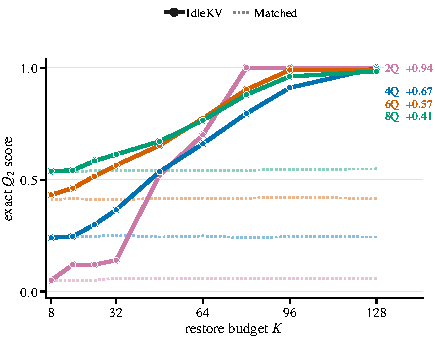
\includegraphics[width=\columnwidth]{figures/frontier_raw_overlay.pdf}
  \caption{Raw exact $Q_2$ score under matched resumed-cache budgets.
  Solid curves are \repairkv{}. Dotted curves are matched no-repair.
  Right labels report query count and $\Delta_{96}$,
  the score gain over matched no-repair at $K=96$.}
  \label{fig:main-frontier}
\end{figure}

\paragraph{Next-turn signal specificity.}
Repair gains are specific to the newly revealed current-turn signal.
At $K=48$, StaleQ-$K$ and WrongQ-$K$ stay near matched no-repair, with
gains $0.028$ $[-0.021,0.083]$ and $[-0.014,0.069]$, while \repairkv{}
reaches $0.326$ $[0.243,0.410]$.
Refresh-buffered's perfect score confirms the right
tokens persist in the active and offloaded keys under matched conditions,
so idle-window repair is feasible in principle. \repairkv{}'s gain over
matched no-repair is preliminary evidence that even a simple
K-promotion selector captures meaningful gains, and designing stronger
selectors is an open research direction.
\begin{table}[t]
  \centering
  \setlength{\tabcolsep}{3.5pt}
  \caption{Next-turn signal specificity at $K=48$ on MQ-NIAH-4Q
  ($72$ paired example-partition cases). Stale and donor controls test
  whether any query-like signal suffices; Refresh is a full-budget
  reselector over active and offloaded KV.}
  \label{tab:specificity-control}
  \begin{tabular}{@{}lcc@{}}
    \toprule
    Condition & $Q_2$ score & $\Delta$ vs.\ matched [95\% CI] \\
    \midrule
    Matched no-repair & $0.215$ & -- \\
    StaleQ-$K$ & $0.243$ & $+0.028$ [$-0.021$, $0.083$] \\
    WrongQ-$K$ & $0.243$ & $+0.028$ [$-0.014$, $0.069$] \\
    \repairkv{} & $0.542$ & $+0.326$ [$0.243$, $0.410$] \\
    Refresh-buffered & $1.000$ & $+0.785$ [$0.722$, $0.847$] \\
    \bottomrule
  \end{tabular}
\end{table}

\paragraph{Repeated relevance shifts.}
The repair effect also survives repeated controlled relevance shifts.
On a fixed five-turn MQ-NIAH-8Q revisit schedule ($K=80$, $n=24$),
\repairkv{} gains $0.542$ over matched no-repair on non-initial turns with
paired bootstrap interval $[0.458,0.620]$.
Random-$K$ and Oldest-$K$
gain only $0.010$ and $0.021$.
\repairkv{} remains above StaleQ-$K$, supporting repeated
cue-conditioned adaptation under controlled relevance shifts.
End-to-end task validation requires trace-based agent benchmarks.
\begin{figure}[tbp]
  \centering
  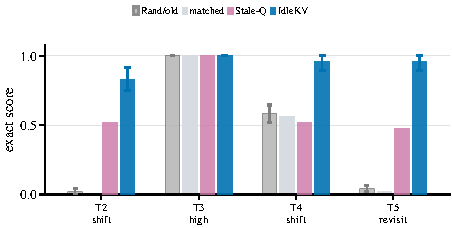
\includegraphics[width=\columnwidth]{figures/multiturn_hard_trajectory.pdf}
  \caption{Five-turn relevance-shift diagnostic on MQ-NIAH-8Q
  ($\bbase{=}18{,}432$, $K{=}80$, $n{=}24$). Groups show post-priming exact
  scores at equal active-cache budget. Intervals are bootstrap $95\%$
  CIs for \repairkv{}, and Stale-Q uses the previous-turn query.}
  \label{fig:multiturn}
\end{figure}

\paragraph{Eviction-policy sensitivity.}
The adaptation effect persists under two protocol-matched compression
policies beyond the primary SnapKV-style policy:
an H$_2$O-style accumulated-attention retention and a
StreamingLLM-style sink-plus-recent rule.
The structurally different sink-plus-recent policy (StreamingLLM-style:
preserve initial sink tokens plus a recent window~\citep{streamingllm})
also passes the gate: at
$K=128$, \repairkv{} gains $0.431$ over matched no-repair while
Random-$K$/Oldest-$K$ remain at the matched baseline.
Canonical reproductions of H$_2$O and StreamingLLM
would require the full original online policies.
A separate Scissorhands-style persistence stress
test~\citep{scissorhands} on MQ-NIAH-6Q also passes the locked gate
(Appendix Table~\ref{tab:app-scissorhands-stress}).
\begin{figure}[t]
  \centering
  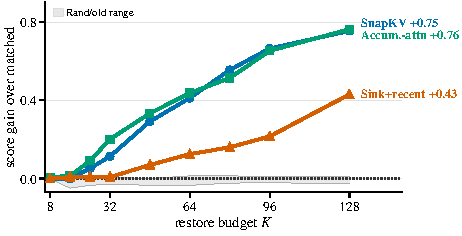
\includegraphics[width=\columnwidth]{figures/policy_breadth_delta.pdf}
  \caption{First-stage eviction-policy sensitivity on MQ-NIAH-4Q
  ($n{=}24$, $\bbase{=}16{,}384$). Curves show exact $Q_2$ gain over each
  policy's matched no-repair baseline. The gray band spans
  Random-$K$/Oldest-$K$ gains.}
  \label{fig:policy-breadth}
\end{figure}

\paragraph{Real-repository diagnostic.}
To test external validity beyond MQ-NIAH, we ran a
controlled real-repository relevance-shift diagnostic on 48 callsite
examples (locations in source where the model must recover a target
identifier such as the called function name) from 12 open-source
repositories drawn from the SWE-bench pool~\citep{swebench} at fixed
commits.
Each example loads 32K tokens of line-numbered file cards from one
repository as the model's context. The first turn $Q_1$ asks about a
file unrelated to the answer, biasing the post-$Q_1$ compression away
from $Q_2$-relevant content so that the answer-bearing tokens are
likely evicted to $W_N$. The second turn $Q_2$ is the callsite
question.
Between turns, an \emph{event} arrives: a description of the
callsite with the target identifier redacted. The event serves as
the next-turn cue $s$ for repair, and all conditions decode the same
event-plus-question prompt (the event followed by a question asking
for the target identifier).
At $K=192$, event-only \repairkv{} (using the event as the only
signal) improves exact identifier accuracy from $18.8\%$ matched to
$72.9\%$.
Non-query controls and ToolFile-$K$ (file-name-assisted: restricts
candidate KV rows to the file named in the event, then backfills
with the oldest evicted rows) remain near matched. File-gated
\repairkv{} (label-assisted: restricts candidates to the file named
in the event) reaches $83.3\%$. AnchorWindow-$K$ (oracle locality
reference: anchors candidates to the ground-truth code region
containing the answer) reaches $89.6\%$.
This remains a small external-validity diagnostic, with no claim to
be a real-code benchmark. Strict exclusions (removing examples where
the matched cache already retained the answer) keep the gain
positive.
Appendix Figure~\ref{fig:app-real-repo-diagnostic} gives the full
audit.
\begin{table}[b]
  \centering
  \setlength{\tabcolsep}{5pt}
  \caption{Preliminary real-repository diagnostic at $K=192$ over $48$
  callsite cases from $12$ open-source repositories
  (SWE-bench pool, fixed commits). Accuracy is
  exact target-identifier recovery. Non-query summarizes the
  best of Random-$K$, Oldest-$K$, StaleQ-$K$, and WrongQ-$K$ analogues. AnchorWindow
  and File-gated are label-assisted; non-label methods are Matched,
  RepairKV, and ToolFile-$K$.}
  \label{tab:real-repo-diagnostic}
  \begin{tabular}{@{}lr@{}}
    \toprule
    Condition & Accuracy \\
    \midrule
    Matched no-repair & $18.8\%$ \\
    Best non-query control & $16.7\%$ \\
    ToolFile-$K$ & $18.8\%$ \\
    \repairkv{} & $72.9\%$ \\
    File-gated \repairkv{} & $83.3\%$ \\
    AnchorWindow-$K$ & $89.6\%$ \\
    \bottomrule
  \end{tabular}
\end{table}

\paragraph{Runtime.}
We run a separate GPU runtime probe for the repair operation.
The probe measures chunked scan, top-$K$ selection, and KV movement over
pinned host-memory BF16 tensors with Qwen-shaped dimensions. At $K=5000$,
p95 repair latency grows from $50.0$\,ms at 32K offloaded candidates to
$1.20$\,s at 1M and $4.64$\,s at 4M (Figure~\ref{fig:runtime-envelope}).
These measurements show the operating range for a single-node GPU
implementation; trace-scheduled serving latency is a natural next systems
step. For context, agent tool calls range from sub-second file/shell
operations to multi-second tasks such as test execution or code
interpretation~\citep{continuum}. Repair at evaluation-relevant offload
sizes (32K--1M rows) fits within these typical tool-call gaps, and longer
windows leave room for larger candidate pools.

\begin{figure}[tbp]
  \centering
  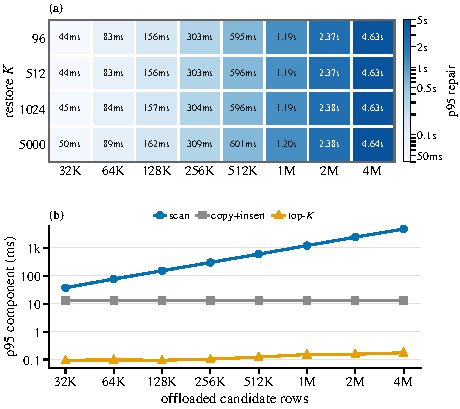
\includegraphics[width=\columnwidth]{figures/runtime_repair_scaling.pdf}
  \caption{Runtime-capacity probe on the evaluation GPU.
  (a) Component-summed p95 service time for chunked scan, top-$K$
  selection, and KV movement at query length 64 over pinned host-memory
  BF16 KV-shaped tensors. (b) Stage-wise p95 component time for $K=5000$.
  Generation and answer evaluation are excluded.}
  \label{fig:runtime-envelope}
\end{figure}

% -----------------------------------------------------------------------
\section{Discussion and Limitations}
\label{sec:discussion}
% -----------------------------------------------------------------------

\repairkv{} is a between-turn maintenance primitive for making KV
compression revisable: a runtime adaptation operator over active KV state
for resource-adaptive tiered-KV runtimes.
It complements existing compression, offload, query-aware access, and
pause/resume serving systems~\citep{vllm,infercept,lmcache,ttkv,
continuum,agentserve} by asking how active memory can be adapted after
compression but before resumed decoding.
The mechanism should be most useful when:
\begin{itemize}[leftmargin=1.4em,noitemsep,topsep=2pt]
  \item the next turn changes which old context matters;
  \item the compressed cache still leaves useful choices in the evicted host-memory store; and
  \item the idle window or scheduler has enough slack for scoring and KV
  movement.
\end{itemize}
The experiments isolate one paused request on one GPU, matching local or
dedicated agent inference but omitting multi-tenant contention.
In shared serving, a scheduler would still need to account for HBM blocks,
copy bandwidth, and queueing slack.
The quality comparisons match active GPU KV budget; total
host-plus-device storage and end-to-end service cost are reported
separately.
The exact-Q$_2$ selector provides a controlled view of the
repair signal, and stronger $Q_2$-aware reselectors, page-level policies,
or full-prefix recompute may further improve the quality-runtime frontier
when enough idle-window slack is available.
The real-repository diagnostic is small and exploratory, so it supports
external validity without serving as a SWE-bench issue-resolution
benchmark.
\paragraph{Conclusion.}
\repairkv{} makes the case for revisable KV compression.
If context relevance changes after eviction, the cache lifecycle can move
in both directions: compress to fit the active budget, then repair by
promoting relevant evicted state before the next decode.
Across MQ-NIAH-2Q/4Q/6Q/8Q, this repair beats matched no-repair while random
and oldest-token promotions stay near baseline.
The broader direction is mutable KV memory for resource-adaptive
long-context inference, with pause windows treated as part of the
inference budget.

\paragraph{Future work.}
Our work highlights the need for a production-facing repair
benchmark that keeps the matched-budget requirements used here, but adds the
features needed to evaluate deployment relevance: multi-turn traces with
explicit pause boundaries, hidden future relevance, shared pre-turn history,
and controls that separate active-cache budget from total storage, transfer,
and recompute cost. It should then test repair across top open and proprietary
long-context models, multiple compression and offload policies, and
production-style traces rather than a single synthetic task family. On the
systems side, the benchmark should measure the idle-window slack available in
real agent workloads such as coding, tool use, retrieval, and browser
interaction, since repair is only useful when scoring and KV movement fit the
scheduler's time and memory constraints. Finally, preliminary nonlinear
variable-tracking diagnostics (Appendix~\ref{app:vt8hop-div2}) suggest that
compression may fail especially sharply when relevant information forms
branching or conflicting dependency graphs rather than linear chains. Turning
that observation into a robust benchmark is a central next step; \repairkv{}
appears robust in preliminary tests, which would further establish the need for a dual compression-repair mechanism, but extensive broader validation is still needed.

\FloatBarrier

% -----------------------------------------------------------------------
\begin{thebibliography}{34}

\bibitem[Abhyankar et~al.(2024)]{infercept}
Abhyankar, R., He, Z., Srivatsa, V., Zhang, H., and Zhang, Y.
\newblock InferCept: Efficient intercept support for augmented large
  language model inference.
\newblock In \emph{Proceedings of the 41st International Conference on
  Machine Learning (ICML)}, 2024.

\bibitem[Bai et~al.(2024)]{longbench}
Bai, Y., Lv, X., Zhang, J., Lyu, H., Tang, J., Huang, Z., Du, Z.,
  Liu, X., Zeng, A., Hou, L., Dong, Y., Tang, J., and Li, J.
\newblock LongBench: A bilingual, multitask benchmark for long context
  understanding.
\newblock In \emph{Proceedings of the 62nd Annual Meeting of the
  Association for Computational Linguistics (ACL)}, 2024.

\bibitem[Bian et~al.(2025a)]{agent_efficiency}
Bian, S., Yan, M., Jayarajan, A., Pekhimenko, G., and Venkataraman, S.
\newblock What limits agentic systems efficiency.
\newblock In \emph{NeurIPS 2025 Workshop on Scaling Environments for
  Agents (SEA)}, 2025.

\bibitem[Bian et~al.(2025b)]{tokencake}
Bian, Z., Wu, F., Ma, T., and Zhuo, Y.
\newblock Tokencake: A KV-cache-centric serving framework for
  LLM-based multi-agent applications.
\newblock \emph{arXiv:2510.18586}, 2025.

\bibitem[Chen et~al.(2025)]{pitfalls}
Chen, A., Geh, R., Grover, A., Van den Broeck, G., and Israel, D.
\newblock The pitfalls of KV cache compression.
\newblock \emph{arXiv:2510.00231}, 2025.

\bibitem[Dzikanyanga et~al.(2026)]{ttkv}
Dzikanyanga, G., Yang, W., Huang, H., Wu, D., Wang, S., Xia, W., and
  K~C, S.
\newblock TTKV: Temporal-tiered KV cache for long-context LLM inference.
\newblock \emph{arXiv:2604.19769}, 2026.

\bibitem[Gao et~al.(2024)]{cachedattention}
Gao, B., He, Z., Sharma, P., Kang, Q., Jevdjic, D., Zhao, J., and
  Zuo, P.
\newblock Cost-efficient large language model serving for multi-turn
  conversations with CachedAttention.
\newblock In \emph{Proceedings of the 2024 USENIX Annual Technical
  Conference (USENIX ATC)}, 2024.

\bibitem[Hsieh et~al.(2024)]{ruler}
Hsieh, C.-Y., Sun, S., Kriman, S., Acharya, S., Rekesh, D., Jia, F.,
  Zhang, Y., and Ginsburg, B.
\newblock RULER: What's the real context window size of your LLM.
\newblock In \emph{Conference on Language Modeling (COLM)}, 2024.

\bibitem[Jimenez et~al.(2024)]{swebench}
Jimenez, C. E., Yang, J., Wettig, A., Yao, S., Pei, K., Press, O.,
  and Narasimhan, K.
\newblock SWE-bench: Can language models resolve real-world GitHub
  issues.
\newblock In \emph{International Conference on Learning
  Representations (ICLR)}, 2024.

\bibitem[Kwon et~al.(2023)]{vllm}
Kwon, W., Li, Z., Zhuang, S., Sheng, Y., Zheng, L., Yu, C. H.,
  Gonzalez, J. E., Zhang, H., and Stoica, I.
\newblock Efficient memory management for large language model serving
  with PagedAttention.
\newblock In \emph{Proceedings of the 29th ACM Symposium on Operating
  Systems Principles (SOSP)}, 2023.

\bibitem[Li et~al.(2024a)]{snapkv}
Li, Y., Huang, Y., Yang, B., Venkitesh, B., Locatelli, A., Ye, H.,
  Cai, T., Lewis, P., and Chen, D.
\newblock SnapKV: LLM knows what you are looking for before generation.
\newblock \emph{arXiv:2404.14469}, 2024.

\bibitem[Li et~al.(2024b)]{pyramidkv}
Li, Z., Yang, Y., Zhang, Y., and Liu, Z.
\newblock PyramidKV: Dynamic KV cache compression based on pyramidal
  information funneling.
\newblock \emph{arXiv:2406.02069}, 2024.

\bibitem[Li et~al.(2025)]{scbench}
Li, Y., Jiang, H., Wu, Q., Luo, X., Ahn, S., Zhang, C., Abdi, A. H.,
  Li, D., Gao, J., Yang, Y., and Qiu, L.
\newblock SCBench: A KV cache-centric analysis of long-context methods.
\newblock In \emph{International Conference on Learning Representations
  (ICLR)}, 2025.

\bibitem[Li et~al.(2026)]{continuum}
Li, H., Mang, Q., He, R., Zhang, Q., Mao, H., Chen, X., Zhou, H.,
  Cheung, A., Gonzalez, J., and Stoica, I.
\newblock Continuum: Efficient and robust multi-turn LLM agent
  scheduling with KV cache time-to-live.
\newblock \emph{arXiv:2511.02230}, 2026.

\bibitem[Liu et~al.(2025)]{lmcache}
Liu, Y., Cheng, Y., Yao, J., An, Y., Chen, X., Feng, S., Huang, Y.,
  Shen, S., Zhang, R., Du, K., and Jiang, J.
\newblock LMCache: An efficient KV cache layer for enterprise-scale LLM
  inference.
\newblock \emph{arXiv:2510.09665}, 2025.

\bibitem[Liu et~al.(2024)]{agentbench}
Liu, X., Yu, H., Zhang, H., Xu, Y., Lei, X., Lai, H., Gu, Y.,
  Ding, H., Men, K., Yang, K., Zhang, S., Deng, X., and others.
\newblock AgentBench: Evaluating LLMs as agents.
\newblock In \emph{International Conference on Learning
  Representations (ICLR)}, 2024.

\bibitem[Liu et~al.(2023)]{scissorhands}
Liu, Z., Desai, A., Liao, F., Wang, W., Xie, V., Xu, Z.,
  Kyrillidis, A., and Shrivastava, A.
\newblock Scissorhands: Exploiting the persistence of importance
  hypothesis for LLM KV cache compression at test time.
\newblock In \emph{Advances in Neural Information Processing Systems
  (NeurIPS)}, 2023.

\bibitem[Qin et~al.(2024)]{toollm}
Qin, Y., Liang, S., Ye, Y., Zhu, K., Yan, L., Lu, Y., Lin, Y.,
  Cong, X., Tang, X., Qian, B., Zhao, S., Hong, L., and others.
\newblock ToolLLM: Facilitating large language models to master
  16000+ real-world APIs.
\newblock In \emph{International Conference on Learning
  Representations (ICLR)}, 2024.

\bibitem[Qwen(2024)]{qwen}
Qwen Team.
\newblock Qwen2.5 technical report.
\newblock \emph{arXiv:2412.15115}, 2024.

\bibitem[Pagonas et~al.(2025)]{cortex}
Pagonas, N., Chung, Y., Kaffes, K., and Krishnamurthy, A.
\newblock Cortex: Workflow-aware resource pooling and scheduling for
  agentic serving.
\newblock \emph{arXiv:2510.14126}, 2025.

\bibitem[Qi et~al.(2026)]{pariskv}
Qi, Y., Chen, X., Jiang, H., Wang, Q., Peng, B., and Palpanas, T.
\newblock ParisKV: Fast and drift-robust KV-cache retrieval for
  long-context LLMs.
\newblock \emph{arXiv:2602.07721}, 2026.

\bibitem[Wu et~al.(2024)]{retrieval_heads}
Wu, W., Wang, Y., Xiao, G., Peng, H., and Fu, Y.
\newblock Retrieval heads mechanistically explain long-context factuality.
\newblock \emph{arXiv:2404.15574}, 2024.

\bibitem[Sun et~al.(2025)]{shadowkv}
Sun, H., Chang, L.-W., Bao, W., Zheng, S., Zheng, N., Liu, X., Dong,
  H., Chi, Y., and Chen, B.
\newblock ShadowKV: KV cache in shadows for high-throughput long-context
  LLM inference.
\newblock \emph{arXiv:2410.21465}, 2025.

\bibitem[Tang et~al.(2024)]{quest}
Tang, J., Zhao, Y., Zhu, K., Xiao, G., Kasikci, B., and Han, S.
\newblock QUEST: Query-aware sparsity for efficient long-context LLM
  inference.
\newblock In \emph{Proceedings of the 41st International Conference on
  Machine Learning (ICML)}, 2024.

\bibitem[Wang et~al.(2025)]{fier}
Wang, D., Liu, Z., Wang, S., Ren, Y., Deng, J., Hu, J., Chen, T., and
  Yang, H.
\newblock FIER: Fine-grained and efficient KV cache retrieval for
  long-context LLM inference.
\newblock In \emph{Proceedings of the Conference on Empirical Methods in
  Natural Language Processing (EMNLP)}, 2025.

\bibitem[Xiao et~al.(2024)]{streamingllm}
Xiao, G., Tang, Y., Zuo, J., Guo, J., Yang, S., Tang, H., Fu, Y.,
  and Han, S.
\newblock Efficient streaming language models with attention sinks.
\newblock In \emph{International Conference on Learning Representations
  (ICLR)}, 2024.

\bibitem[Zhang et~al.(2023)]{h2o}
Zhang, Z., Sheng, Y., Zhou, T., Chen, T., Zheng, L., Cai, R., Song, Z.,
  Tian, Y., R{\'e}, C., Barrett, C., Wang, Z., and Chen, B.
\newblock H$_2$O: Heavy-hitter oracle for efficient generative inference
  of large language models.
\newblock In \emph{Advances in Neural Information Processing Systems
  (NeurIPS)}, 2023.

\bibitem[Zhang et~al.(2024)]{inftybench}
Zhang, X., Chen, Y., Hu, S., Xu, Z., Chen, J., Hao, M. K., Han, X.,
  Thai, Z. L., Wang, S., Liu, Z., and Sun, M.
\newblock $\infty$Bench: Extending long context evaluation beyond 100K
  tokens.
\newblock In \emph{Proceedings of the 62nd Annual Meeting of the
  Association for Computational Linguistics (ACL)}, 2024.

\bibitem[Zhang et~al.(2025)]{lazy_eviction}
Zhang, H., Zhang, H., Ma, X., Zhang, J., and Guo, S.
\newblock LazyEviction: Lagged KV eviction with attention pattern
  observation for efficient long reasoning.
\newblock \emph{arXiv:2506.15969}, 2025.

\bibitem[Zhang et~al.(2026)]{agentserve}
Zhang, Y., Yan, Y., Yang, N., and Yuan, D.
\newblock AgentServe: Algorithm-system co-design for efficient agentic
  AI serving on a consumer-grade GPU.
\newblock \emph{arXiv:2603.10342}, 2026.

\bibitem[Zheng et~al.(2026)]{agentcgroup}
Zheng, Y., Fan, J., Fu, Q., Yang, Y., Zhang, W., and Quinn, A.
\newblock AgentCgroup: Understanding and controlling OS resources of AI
  agents.
\newblock \emph{arXiv:2602.09345}, 2026.

\bibitem[Zhou et~al.(2024)]{webarena}
Zhou, S., Xu, F. F., Zhu, H., Zhou, X., Lo, R., Sridhar, A.,
  Cheng, X., Ou, T., Bisk, Y., Fried, D., Alon, U., and Neubig, G.
\newblock WebArena: A realistic web environment for building autonomous
  agents.
\newblock In \emph{International Conference on Learning
  Representations (ICLR)}, 2024.

\end{thebibliography}

\newpage
\appendix
\onecolumn
\raggedbottom

\section{Additional Evaluation Details}
\label{app:evaluation-details}

\paragraph{Protocol details.}
Concise split prompts request values only, comma-separated, with a short
answer prefix and fixed decode budgets of 24 tokens for MQ-NIAH-4Q,
48 tokens for MQ-NIAH-6Q, and 64 tokens for MQ-NIAH-8Q.
Generation is deterministic greedy decoding with no sampling.
The main examples use dataset seed offset 0.
Random-$K$ uses a
deterministic example- and $K$-dependent seed.
Bootstrap intervals are percentile intervals over paired
example-partition rows with fixed seeds.
Main Qwen runs use BF16 weights on one RTX PRO 6000 Blackwell GPU with
Python 3.12.3, PyTorch 2.10.0+cu128, and Transformers 5.2.0.
The exact-Q$_2$ attention-query selector appends $Q_2$ to
the compressed active cache, extracts the model's post-RoPE query
projections for the $Q_2$ prompt tokens, and scores active and offloaded
key rows under those projections before selecting evicted rows for
promotion. This selector is distinct from decode-time answer-token
attention and from the final answer metric. The $Q_2$-appended-state proxy
appends $Q_2$ to the compressed cache and uses the appended cache rows as
a second Q$_2$-conditioned scoring signal.

\paragraph{Span-group diagnostic.}
\spanref{} starts from the same $B$ state and offloaded evicted-KV store
as \repairkv{}.
It enumerates the small family of annotated $Q_2$ answer-span-group
subsets, one key/value span group per requested needle, evaluates each
subset once under actual $Q_2$ generation, and chooses the
highest-scoring subset with total cost at most $K$.
It is exact over this benchmark-specific span-group family, but not over
all arbitrary token subsets or possible final generations.
Because the selected span-group subset may use fewer than $K$ rows, a
repair selector can occasionally score higher at low budgets by spending
the full budget on useful local neighborhoods around future-relevant
spans. Thus \spanref{} is a diagnostic span-group reference, not a
ceiling. 

\paragraph{Partition choices.}
For MQ-NIAH-4Q, the pooled panel uses
$14{\rightarrow}23$, $24{\rightarrow}13$, and
$34{\rightarrow}12$.
These are the balanced $2|2$ partitions whose $Q_2$ side excludes the
tail-anchored fourth needle.
For MQ-NIAH-6Q, the pooled panel uses
$156{\rightarrow}234$, $256{\rightarrow}134$,
$356{\rightarrow}124$, and $456{\rightarrow}123$, so the second turn
excludes the two latest needles.
For MQ-NIAH-8Q, the pooled panel uses
$5678{\rightarrow}1234$, $1678{\rightarrow}2345$,
$2678{\rightarrow}1345$, $3678{\rightarrow}1245$, and
$4678{\rightarrow}1235$, again excluding the two latest needles from the
second turn.
Within-turn order is not treated as a separate condition because the
prompt asks for comma-separated values only and scoring checks whether
each requested value is recovered.
Recency-favorable splits such as $12{\rightarrow}34$ are left to
separate diagnostics outside the main future-query repair result.

\paragraph{Scissorhands-style persistence stress test.}
Table~\ref{tab:app-scissorhands-stress} repeats the MQ-NIAH-6Q locked
protocol after replacing the initial SnapKV-style eviction policy with a
one-shot persistence policy inspired by Scissorhands.
The test asks whether repair still works when the compressed active cache
is chosen by past attention persistence in place of the primary eviction
policy.
Canonical online per-head Scissorhands reproduction remains future work.

\begin{table}[H]
  \centering
  \caption{Scissorhands-style persistence stress test on
  MQ-NIAH-6Q ($\bbase{=}18{,}432$, $n{=}24$). Values are exact scores. Best
  ctrl. is the stronger of Random-$K$ and Oldest-$K$; the interval is the
  paired bootstrap $95\%$ CI for \repairkv{}$-\bmatch$.}
  \label{tab:app-scissorhands-stress}
  \small
  \begin{tabular}{rrrrrr}
    \toprule
    $K$ & Full & $\bmatch$ & Best ctrl. & \repairkv{} & Gain CI \\
    \midrule
    48 & 0.990 & 0.365 & 0.382 & 0.712 & [0.292, 0.403] \\
    64 & 0.990 & 0.365 & 0.382 & 0.795 & [0.378, 0.490] \\
    80 & 0.990 & 0.378 & 0.385 & 0.934 & [0.503, 0.604] \\
    96 & 0.990 & 0.375 & 0.382 & 0.993 & [0.566, 0.670] \\
    128 & 0.990 & 0.368 & 0.378 & 0.990 & [0.573, 0.674] \\
    \bottomrule
  \end{tabular}
\end{table}

\section{Additional Discussion}
\label{app:additional-discussion}

\paragraph{Tiered-cache scaling.}
Repair creates a two-level cache-budget problem because the main curves match
the resumed active GPU KV budget while tracking total host-plus-device
storage separately.
A strict device-resident policy chooses the active-cache budget, while a
looser off-device policy decides which evicted rows remain searchable,
compressed, summarized, or recomputable.
In the Qwen-shaped accounting
above, 4M searchable rows already imply about 240\,GB before metadata.
Thus \repairkv{} supports the middle operation in a tiered hierarchy:
turn-conditioned promotion from host memory during an idle window.
This is a hardware-facing implication; hardware measurement remains
future work.

\paragraph{Idle-window repair interface.}
A practical implementation would expose a host-memory index over evicted KV
units, a time-budgeted selector conditioned on the next-turn signal,
asynchronous promotion into the active cache, and fallbacks to no-repair or
full recompute.
This turns a pause into a schedulable resource: the system can spend only
the slack that remains after queueing, transfer, and generation
constraints, and can move the selector from token rows to pages or
compressed metadata as hardware and serving constraints require.

\paragraph{Preliminary nonlinear variable-tracking diagnostic.}
\label{app:vt8hop-div2}
As an exploratory stress test, we also tested a modified RULER
variable-tracking task that makes the dependency structure less linear than the
standard 4-hop chain. The diagnostic uses an 8-hop permuted chain with two
distractor divergences: some assignments introduce branches that are not used by
the final answer, so the model must recover the relevant path through a small
information graph rather than follow a tail-friendly linear sequence. In
32K-context Qwen2.5-7B-Instruct runs, SnapKV compression degraded this task
sharply even at moderate retained-cache budgets. Preliminary repair runs
recovered substantial accuracy from the same compressed states using small
restore fractions. These results are not part of the main evidence, but they
motivate a broader benchmark for nonlinear and conflicting relevance patterns,
where eviction policies may fail even when standard long-context tasks appear
solved.

\paragraph{Future benchmark axes.}
Future benchmarks should vary the number, timing, and conflict structure
of new-turn constraints.
The 2Q and 8Q breadth checks suggest that easy regimes can saturate while
stricter multi-query turns expose how quickly eviction failures
accumulate.
The five-turn diagnostic strengthens the dynamic-workflow evidence, but
it remains synthetic.
Broader task families should keep the same
matched-budget controls while adding real tool traces and stronger
selector families.

\section{Supplementary Experimental Views}
\label{app:supplementary-figures}

The supplementary figures probe external validity,
query-count and operating-regime breadth, partition consistency, runtime
capacity, and appendix selector diagnostics.
Exact audit values remain in released result artifacts.
\FloatBarrier

\IfFileExists{figures/real_repo_repair_diagnostic.pdf}{%
\begin{figure}[H]
  \centering
  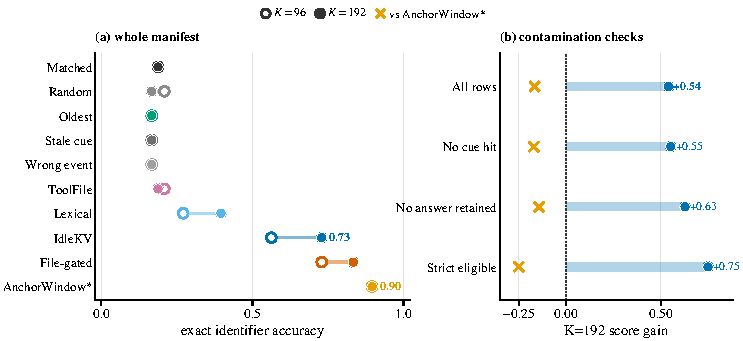
\includegraphics[width=0.94\textwidth]{figures/real_repo_repair_diagnostic.pdf}
  \caption{Controlled real-repository relevance-shift diagnostic over
  $48$ callsite examples from $12$ repositories drawn from the SWE-bench
  repository pool at pinned commits. Repair sees only the event cue. All
  conditions decode the same event-plus-question prompt. Left: exact
  identifier accuracy at $K=96$ and $K=192$. Right: $K=192$ \repairkv{}
  gain over matched no-repair after removing cue-only or answer-retention
  rows. ToolFile-$K$ is file-name-assisted with oldest-row backfill.
  File-gated \repairkv{} restricts candidates to the event-named file before
  applying the event-only scorer. Lexical is an answer-sanitized diagnostic
  outside the deployable-selector comparison.
  AnchorWindow-$K$ is a label-assisted locality reference outside the
  deployable-baseline and end-to-end issue-resolution comparisons.}
  \label{fig:app-real-repo-diagnostic}
\end{figure}
}{}

\IfFileExists{figures/query_count_breadth.pdf}{%
\IfFileExists{figures/operating_regime_heatmap.pdf}{%
\begin{figure}[H]
  \centering
  \begin{minipage}[t]{0.35\textwidth}
    \vspace{0pt}
    \centering
    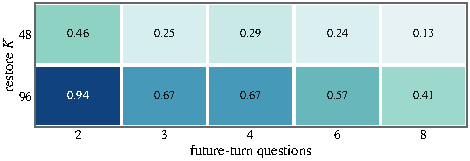
\includegraphics[width=\linewidth]{figures/query_count_breadth.pdf}\\[-0.35em]
    {\small (a) Query-count breadth}
  \end{minipage}\hfill
  \begin{minipage}[t]{0.59\textwidth}
    \vspace{0pt}
    \centering
    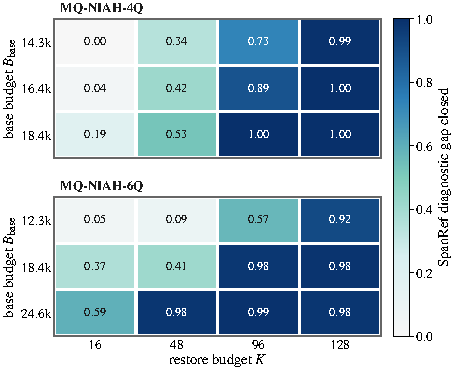
\includegraphics[width=\linewidth]{figures/operating_regime_heatmap.pdf}\\[-0.35em]
    {\small (b) Operating regime}
  \end{minipage}
  \caption{Supplementary breadth diagnostics. (a) Cells show \repairkv{}
  score gain over matched no-repair for $K=48$ and $K=96$ across
  2-, 3-, 4-, 6-, and 8-question split-query variants. (b) Cells show the
  fraction of available \spanref{} diagnostic gain recovered by \repairkv{},
  clipped to $[0,1]$, for MQ-NIAH-4Q/6Q. Saturated cells with little
  matched-to-\spanref{} gap should not be read as upper-bound statements.}
  \label{fig:app-breadth-operating}
\end{figure}
}{}}{}

\IfFileExists{figures/partition_endpoint_dotplot.pdf}{%
\begin{figure}[H]
  \centering
  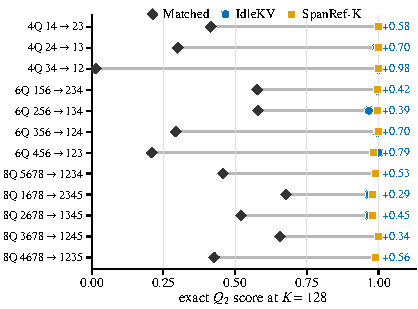
\includegraphics[width=0.74\textwidth]{figures/partition_endpoint_dotplot.pdf}
  \caption{Per-partition endpoint scores at $K=128$ on the final exact
  evaluations. Gray segments show the change from matched
  no-repair to \repairkv{}, orange points show the benchmark-metadata
  \spanref{} diagnostic, and labels report the \repairkv{} difference over
  matched no-repair.}
  \label{fig:app-partition-endpoints}
\end{figure}
}{}

\IfFileExists{figures/repair_selection_diagnostic.pdf}{%
\begin{figure}[H]
  \centering
  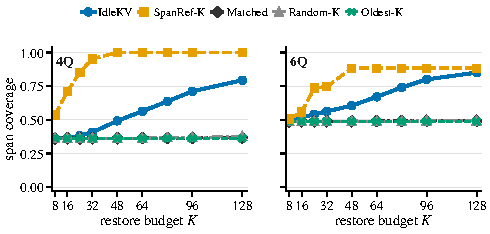
\includegraphics[width=\columnwidth]{figures/repair_selection_diagnostic.pdf}
  \caption{Mechanism diagnostic for the final exact MQ-NIAH evaluations.
  Curves show overlap between promoted tokens and annotated $Q_2$ answer
  spans. Content-agnostic promotions stay near baseline while \repairkv{}
  increasingly covers future-relevant spans.}
  \label{fig:selection-diagnostic}
\end{figure}
}{}

\IfFileExists{figures/runtime_capacity_curve.pdf}{%
\IfFileExists{figures/proxy_controlled_frontier.pdf}{%
\begin{figure}[H]
  \centering
  \begin{minipage}[t]{0.48\textwidth}
    \vspace{0pt}
    \centering
    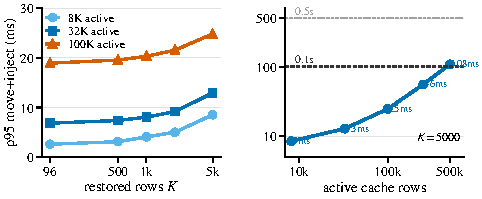
\includegraphics[width=\linewidth]{figures/runtime_capacity_curve.pdf}\\[-0.35em]
    {\small (a) Move-and-inject capacity}
  \end{minipage}\hfill
  \begin{minipage}[t]{0.48\textwidth}
    \vspace{0pt}
    \centering
    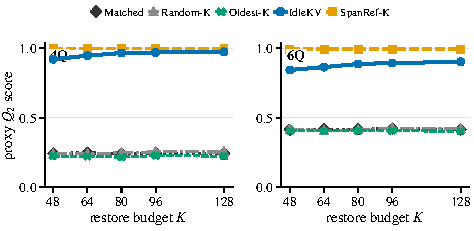
\includegraphics[width=\linewidth]{figures/proxy_controlled_frontier.pdf}\\[-0.35em]
    {\small (b) Proxy-selector diagnostic}
  \end{minipage}
  \caption{Supplementary runtime and selector diagnostics.
  (a) Synthetic move-and-inject capacity for Qwen-shaped BF16 KV on the
  evaluation GPU, separate from the Figure~\ref{fig:runtime-envelope}
  scan/select envelope. Measurements use pinned host-memory promoted
  blocks and report p95 latency as $K$ or active cache size grows.
  (b) Appendix proxy-selector diagnostic on MQ-NIAH-4Q/6Q ($100$ examples
  per split). At $K=96$, content-agnostic promotions stay within
  $0.010$/$0.004$ of matched no-repair while proxy \repairkv{} remains
  well above matched.}
  \label{fig:app-runtime-capacity}
  \label{fig:app-proxy-controlled}
\end{figure}
}{}}{}

\end{document}
